\section{Pregunta N$^{\circ}$12\qquad León Alonzo Terrones Caccha}

\begin{frame}
    \begin{enumerate}\setcounter{enumi}{11}
        \item

              El problema de valor inicial

              \begin{equation*}
                  \begin{cases}
                      \diff{y}{t}=\exp\left(y\left(t\right)\right)
                                         &
                      t\in\left[0,0.20\right]. \\
                      y\left(0\right)=1, &
                  \end{cases},
              \end{equation*}
              tiene solución
              \begin{math}
                  y\left(t\right)=
                  1-\ln\left(1-et\right)
              \end{math}.
              Aplique el método de Adams-Moulton de tres pasos.
    \end{enumerate}

    \begin{solution}
        \begin{figure}[ht!]
            \centering
            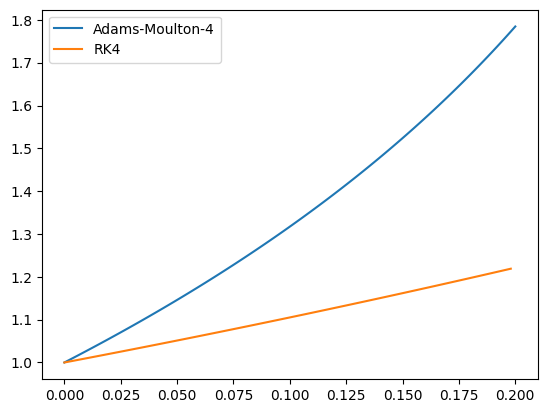
\includegraphics[width=.55\paperwidth]{p12-Comparar-results.png}
        \end{figure}
    \end{solution}
\end{frame}

\begin{frame}
    \begin{figure}[ht!]
        \centering
        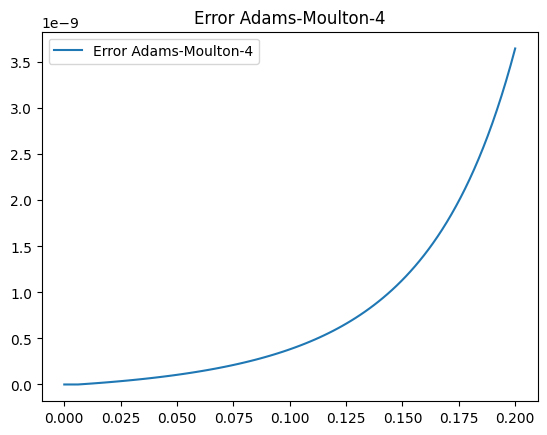
\includegraphics[width=.7\paperwidth]{p12-Error-AM.png}
    \end{figure}
\end{frame}

\begin{frame}
    \begin{figure}[ht!]
        \centering
        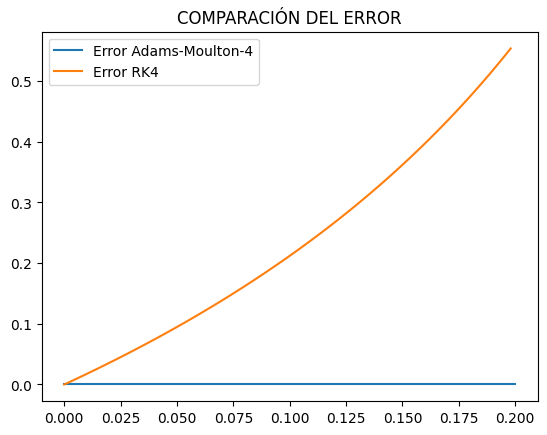
\includegraphics[width=.7\paperwidth]{p12-Comp-error.png}
    \end{figure}
\end{frame}